\documentclass[pdf]{beamer}

\RequirePackage[utf8]{inputenc}
\RequirePackage[T1]{fontenc}
\RequirePackage{lmodern}

% for speaker notes etc
\RequirePackage{pgfpages}
%\setbeameroption{show notes on second screen}
%\setbeameroption{show only notes}
\setbeamercolor{note page}{bg=white}
\setbeamercolor{note title}{bg=white!90!black, fg=black}
\setbeamercolor{note date}{parent=note title}

\beamertemplatenavigationsymbolsempty
\AtBeginSection[]{
    \begin{frame}
        \vfill
        \centering
        \begin{beamercolorbox}[sep=8pt,center,shadow=true,rounded=true]{title}
            \usebeamerfont{title}\insertsectionhead\par%
        \end{beamercolorbox}
        \vfill
    \end{frame}
}

\RequirePackage{listings}
\lstset{escapeinside={<@}{@>}}
\lstset{basicstyle=\ttfamily}
\lstset{moredelim=**[is][\color{red}]{@}{@}}

\RequirePackage{dirtree}
\RequirePackage{csquotes}

\RequirePackage{minted}
\setminted{fontsize=\scriptsize}


\mode<presentation>{}

\title{Building C++-Python libraries}
\subtitle{}
\author{Jørgen Kvalsvik <jokva@equinor.com>}
\titlegraphic{
\includegraphics[width=0.33\textwidth]{equinor-red.eps}}

\begin{document}

% title-page + title-page notes
\maketitle
\note {
    \begin{itemize}
        \item Introduce me and my team
        \item Python is pretty good at high-level problem description
        \item We still want to do the heavy lifting in C++
        \item Good examples are tensorflow, scikit-learn, numpy
        \item Our colleagues use python, and want us to provide ready-to-use
              packages
        \item Then you need to \emph{build} then, and we have made some painful
              experiences with that
    \end{itemize}
}

\begin{frame}{Outline}
    \tableofcontents
\end{frame}

\begin{frame}
    \begin{center}
        
\includegraphics[keepaspectratio, height = 0.8\textheight]{Mechazawa.png}
    \end{center}
\end{frame}

\section{Kinds}
\begin{frame}
    python3 -m pip install my-project

    \note {
        This is the only end-user code in this talk. The rest is of it is all
        developer centric
    }
\end{frame}

\begin{frame}{Kinds of Python}
    \begin{itemize}
        \item Pure python
        \item Impure python (non-python backend)
        \item Thin library wrappers
        \item Fat library wrappers
    \end{itemize}

    \note{
        \begin{itemize}
            \item Pure python is what we want out downstream users to do
            \item Impure python is almost indistinguishable from pure python:
                  Numpy and chunks of the python standard library are good
                  examples
            \item Thin wrappers rely on some system provided library and
                  provide an entry point from Python. Fire, wait, and parse the
                  output
            \item Rely on larger,  but do more than just provide an entry point
                  - sophisticated I/O, manipulation of state, and rich access
                  to library functionality. Difference between this and impure
                  python is that numpy's backend is only available in python,
                  contrary to say python-BLAS
        \end{itemize}
        We'll focus on impure and fat library
    }
\end{frame}

\begin{frame}
    \begin{block}{}
        What does pip install do?
    \end{block}
\end{frame}

\begin{frame}
    \begin{enumerate}
        \item Looks up the package name in an \emph{index}
        \item Determines if the package is installable
        \item Fetches the package
        \item Extracts the package site-packages/
    \end{enumerate}
\end{frame}

\begin{frame}
    \begin{center}
    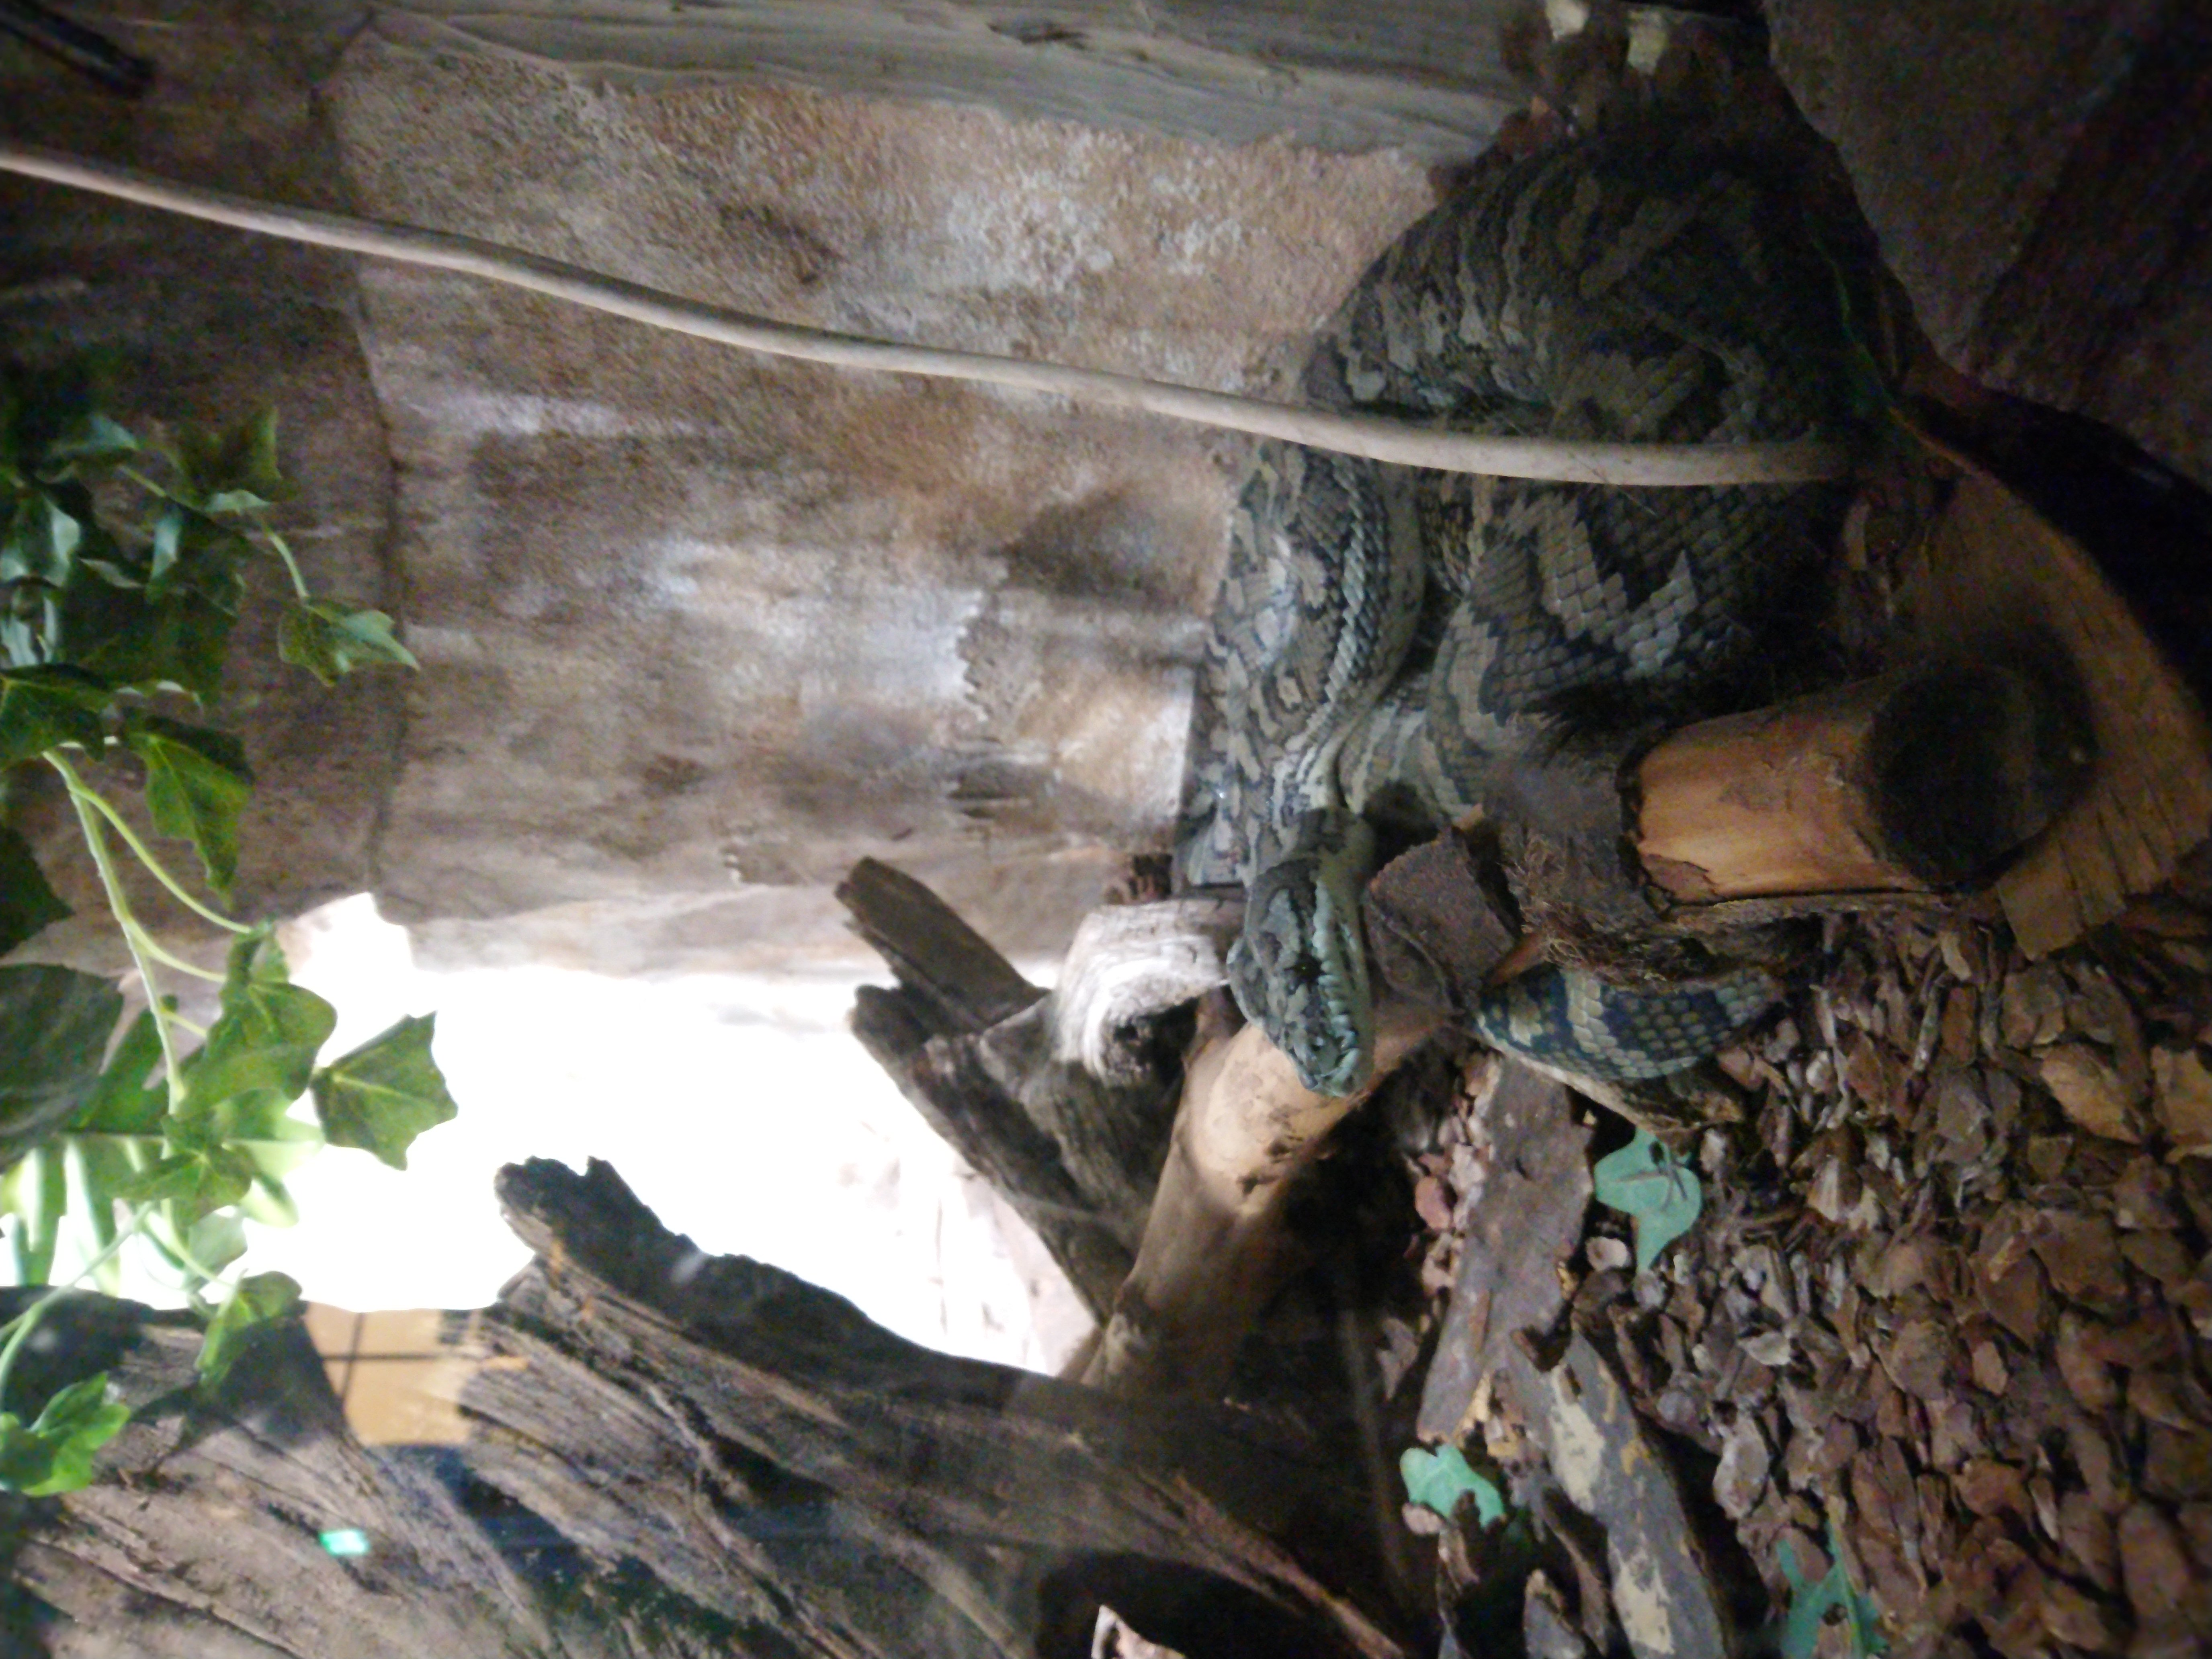
\includegraphics[keepaspectratio, height = 0.9\textheight]{snake.jpg}
    \end{center}
    \note {
        This is a Python package, or rather, a packaged Python
    }
\end{frame}

\section{What's in a package?}
\begin{frame}
    Python is interpreted on the fly

    \note{
        \begin{itemize}
            \item We still talk about \emph{building} packages even though it's
                  a glorified directory copy
            \item To shed some light on it, let's look at the internals of your
                  run-of-the-mill python project
        \end{itemize}
    }
\end{frame}

\begin{frame}{Mechazawa's project}
    \dirtree{%
        .1 project/.
        .2 README.rst.
        .2 LICENSE.
        .2 setup.py.
        .2 requirements.txt.
        .2 my-package/.
        .3 {\_\_}init{\_\_}.py.
        .3 core.py.
        .3 helpers.py.
        .2 docs/.
        .3 conf.py.
        .3 index.rst.
        .2 tests/.
        .3 test{\_}basic.py.
        .3 test{\_}advanced.py.
    }

    {\tiny https://docs.python-guide.org/writing/structure}
    \note{
        \begin{itemize}
            \item This is a source tree listing, a git checkout or similar
            \item Building this package is essentially just copying the
                  package/ directory to the correct python/site-packages
            \item Sometimes you want to do some pre-processing to source files,
                  pre-set variables depending on system, bundle data files etc
        \end{itemize}
    }
\end{frame}

\begin{frame}[fragile]
    \begin{minted}{bash}
$ python3 setup.py bdist_wheel
$ unzip -l dist/my_project-0.0.1-py3-none-any.whl
my_package/__init__.py
my_package/core.py
my_package/helpers.py
my_project-0.0.1.dist-info/LICENSE
my_project-0.0.1.dist-info/METADATA
my_project-0.0.1.dist-info/WHEEL
my_project-0.0.1.dist-info/top_level.txt
my_project-0.0.1.dist-info/RECORD
    \end{minted}
\end{frame}

\begin{frame}
    \dirtree{%
        .1 site-packages/.
        .2 my-package/.
        .3 {\_\_}init{\_\_}.py.
        .3 core.py.
        .3 helpers.py.
        .2 numpy/.
        .2 pandas/.
        .2 minisat/.
    }

    \note{
        \begin{itemize}
            \item Both the previous examples, when built and install, end up
                  like this
        \end{itemize}
    }
\end{frame}

\begin{frame}
    
\includegraphics[width=\textwidth]{pantheon.jpeg}
    \note{
        \begin{itemize}
            \item Anyone know what this is?
            \item Important to understand how we got here
        \end{itemize}
    }
\end{frame}

\section{History}
\begin{frame}
    \begin{description}
        \item [Late 90s] Python wanted something like CPAN
        \item [2000] Distutils released for Python 1.6 standard library
        \item [2003] PyPI is online, distutils can create package metadata
        \item [2008] Setuptools extends and replaces distutils
        \item [2008] pip builds on setuptool
    \end{description}

    \note{
        \emph{Read the list}: standard library is where modules go to die
        \begin{itemize}
            \item Setup written for distutils generally work with setuptools,
                  strong backwards compatibility. This also means a lot of
                  legacy
            \item Distutils came with infrastructure for building C code, a
                  uses homegrown compiler abstraction
            \item Assumes the same compiler that built Python is available
            \item This is terrible on Windows where dealing with compilers is a
                  pain
            \item No custom options really, stuck on the configuration
                  setuptools already has
            \item Building pollutes source tree
            \item Let's start building a package
        \end{itemize}
    }
\end{frame}

\section{Using setuptools}
\begin{frame}[fragile]
    \inputminted{python}{my-package/setuptools-pure.py}

    \note{
        \begin{itemize}
            \item This is for a pure python package
            \item It's quite minimal, setuptools support a wide range of keys
                  and metadata. It can figure some things out, since our
                  project is \emph{standard layout}
            \item Let's write some native code, a C extension
        \end{itemize}
    }
\end{frame}

\begin{frame}[fragile]
    \inputminted[highlightlines=11]{python}{my-package/setuptools-ext.py}
\end{frame}

\begin{frame}[fragile]
    \inputminted{c}{my-package/my_package/math/math.c}
\end{frame}

\begin{frame}[fragile]{}
    \begin{minted}{python}
>>> import my_package
>>> my_package.math.add(1, 2)
3
    \end{minted}
    \note {
        \begin{itemize}
            \item This extension is, of course, trivial
            \item Let's spice it up and use C++11
        \end{itemize}
    }
\end{frame}

\begin{frame}[fragile]
    \inputminted[
        highlightlines={3,6}
    ]{c++}{my-package/my_package/math/math11.cpp}

    \note{
        \begin{itemize}
            \item This now fails on gcc < 6.0, because C++98 was still the
                  default
            \item Of course it's still valid C++, so it just needs the option
        \end{itemize}
    }
\end{frame}

\begin{frame}[fragile]
    \inputminted{python}{my-package/setuptools-ext11.py}

    \note{
        \begin{itemize}
            \item Ok good, so this builds... on linux
            \item MSVC doesn't understand this flag
            \item So now our script needs to detect compiler and only set the
                  flag on gcc
            \item ... until we also want to build with clang
            \item If you've ever built C++ for multiple platforms or even
                  different computers you see how this can get problematic fast
            \item It's quite hard to ad-hoc configure on new systems
        \end{itemize}
    }
\end{frame}

\begin{frame}[fragile]
    \begin{minted}{python}
extra_compile_args = []
if 'win' not in sys.platform:
    extra_compile_args.append('-std=c++11')

my_math = setuptools.Extension('my_package.math',
    sources = ['my_package/math/math11.cpp'],
    extra_compile_args = extra_compile_args,
)
    \end{minted}
\end{frame}

\begin{frame}[fragile]
    \begin{minted}{bash}
$ python3 setup.py build_ext --help

Options for build_ext command:
    --library-dirs (-L)  directories to search for external C libraries
                         (separated by ':')
    \end{minted}
\end{frame}

\begin{frame}
    \begin{center}
        
\includegraphics[height = 0.8\textheight]{mechazawa-sad.jpg}
    \end{center}
\end{frame}

\begin{frame}
    \begin{center}
        \includegraphics[height = 0.8\textheight]{scream.jpg}
    \end{center}
\end{frame}

\section{And then things got worse ...}

\begin{frame}{The struggle of binary libraries}
    \begin{itemize}
        \item Compiler options
        \item Compiler versions
        \item Choosing the right compiler
        \item Platform-specific options
        \item Binary compatibility
    \end{itemize}
\end{frame}

\begin{frame}[fragile]{The struggle of binary libraries}
    \begin{description}
        \item [Configuration-specific] \verb|USE_BLAS|
        \item [Header detection] \verb|#include| sys/inet.h or winsock.h
        \item [Dependencies] Build time
        \item [Dependencies] Runtime
    \end{description}

    \note{
        \emph{Read list}
        \begin{itemize}
            \item The experience compiling and developing native extensions is
                  terrible
            \item Setuptools has virtually nothing to help you here, boils down
                  to manually implementing half of cmake
            \item The development story is quite bad too
            \item People end up hard-coding links to /opt/local/lib64, I can't
                  blame them
            \item Since setup.py implements build, install, test commands,
                  custom option commands are difficult or clumsy
        \end{itemize}
    }
\end{frame}

\begin{frame}
    \inputminted{c++}{my-package/template-div1.cpp}
\end{frame}

\begin{frame}[fragile]
    \begin{minted}{python}
>>> my_package.math.div(4, 2)
1
    \end{minted}
\end{frame}

\begin{frame}[fragile]
    \begin{minted}{python}
>>> my_package.math.div(2, 0)
    \end{minted}
\end{frame}

\begin{frame}
    \inputminted{c++}{my-package/template-div2.cpp}
\end{frame}

\begin{frame}[fragile]
    \verb|$ python3 setup.py build|
    \note{
        \begin{itemize}
            \item Overall, setuptools does a poor job of tracking file ->
                  compiled object dependencies
            \item Not designing for live development of C based modules is
                  fine, they weren't aiming to build a C build system. But most
                  time is spent is development (by me), and having parallel
                  development and build systems suck
        \end{itemize}
    }
\end{frame}

\begin{frame}{Is paradise lost?}
    \begin{center}
    
\includegraphics[keepaspectratio, height = 0.8\textheight]{fall-of-lucifer.jpg}
    \end{center}
    \note{
        \begin{itemize}
            \item The talk name did hint of a solution
            \item A lot of installed stuff is happy to hard-code path to python
                  exe + libs
        \end{itemize}
    }
\end{frame}

\section{A new tomorrow}

\begin{frame}
    \begin{displayquote}
        The scikit-build package is fundamentally just glue between the
        setuptools Python module and CMake
    \end{displayquote}
    - scikit-build readme

    \note{
        \begin{itemize}
            \item Briefly, it automates building C++ with cmake
            \item It adresses most of the shortcomings with setuptools for
                  extensions
            \item Setuptools does what setuptools can (build python), cmake
                  does what cmake does
        \end{itemize}
    }
\end{frame}

\begin{frame}[fragile]
    \begin{itemize}
        \item \verb|find_package|
        \item \verb|target_link_libraries|
        \item \verb|set(CMAKE_CXX_STANDARD)|
        \item \verb|if (MSVC)|
    \end{itemize}

    \note{
        \begin{itemize}
            \item Hate it or love it, cmake is pretty good at what it does
            \item It's reasonably easy to set options, deal with compiler
                  differences in cmake
            \item When you have third-party dependencies that provide
                  cmake-config or similar, you can easily get them from inside
                  the python extension with find-package
            \item cmake is pretty good at dealing with platform differences
        \end{itemize}
    }
\end{frame}

\begin{frame}
    \begin{itemize}
        \item Configuration-specific configuration
        \item Header detection
        \item Dependencies build time
        \item Dependencies runtime
    \end{itemize}
\end{frame}

\begin{frame}[fragile]
    \begin{tabular}{l l}
        Configuration-specific  & \verb|if (BUILD_PYTHON)| \\
        Header detection        & \verb|check_include_file(sys/stat.h)| \\
        Build                   & \verb|find_package(FLEX)| \\
        Runtime                 & \verb|target_link_libraries(lib)| \\
    \end{tabular}
\end{frame}

\begin{frame}[fragile]
    \inputminted{python}{my-package/scikit-build.py}

    \note {
        \begin{itemize}
            \item It does support of a few scikit-build specific keys, like
                  cmake-args, but other than that mostly just setuptools
        \end{itemize}
    }
\end{frame}

\begin{frame}[fragile]
    \inputminted{cmake}{my-package/CMakeLists.txt}

    \note {
        \begin{itemize}
            \item The PythonExtensions module is provided by scikit-build
            \item This is really it. It works quite well, and the maintainers
                  are helpful
            \item Ok, but let's pretend we want to also link against zlib
        \end{itemize}
    }
\end{frame}

\begin{frame}[fragile]
    \inputminted[highlightlines={6, 10}]{cmake}{my-package/CMakeLists-zlib.txt}
    \note{
        \begin{itemize}
            \item All we had to do was find-package and target-link-libraries
            \item We outsource the dealing with platforms, linking and
                  detection to cmake
            \item The python build script is unaware - this is all a detail
                  of the extension anyway
            \item Let's assume that on the dev machine, zlib is installed in a
                  non-standard location
        \end{itemize}
    }
\end{frame}

\begin{frame}[fragile]
    \verb|python3 setup.py build -- -DZLIB_DIR=~/.local/zlib|

    \note {
        \begin{itemize}
            \item scikit-build allows easy access to cmake configuration
            \item unlike setuptools before, because scikit-build actually
                  extended argument parsing
            \item Now we can easily configure the library without changing
                  build script code
        \end{itemize}
    }
\end{frame}

\begin{frame}
    \inputminted{c++}{my-package/template-div2.cpp}
\end{frame}

\section{Intermezzo: cmake integration}
\begin{frame}[fragile]

    \verb|mkdir build && cd build && cmake ..|
    \verb|make && ctest --output-on-failure|

    \note{
        \begin{itemize}
            \item This command is really what I mostly do during development
            \item It builds the core libraries, some applications, the python
                  extension, the python library, and docs if enabled
            \item And runs the tests, across all languages
            \item It uses relies on setup.py to build and test python
        \end{itemize}
    }
\end{frame}

\begin{frame}
    Avoid double bookkeeping
\end{frame}

\begin{frame}
    \dirtree{%
        .1 project/.
        .2 CMakeLists.txt.
        .2 core/.
        .3 CMakeLists.txt.
        .3 core.cpp.
        .2 python/.
        .3 CMakeLists.txt.
        .3 setup.py.
        .3 my-package/.
        .2 haskell/.
        .3 CMakeLists.txt.
        .3 core.hs.
    }
\end{frame}

\begin{frame}
    \dirtree{%
        .1 project/.
        .2 CMakeLists.txt.
        .2 core/.
        .3 CMakeLists.txt.
        .3 core.cpp.
        .2 python/.
        .3 {\color{red}{CMakeLists.txt}}.
        .3 setup.py.
        .3 my-package/.
        .2 haskell/.
        .3 CMakeLists.txt.
        .3 core.hs.
    }
\end{frame}

\begin{frame}[fragile]
    \inputminted{cmake}{my-package/custom-target.cmake}

\note{
    \begin{itemize}
        \item If you're not familiar with cmake or custom targets, it makes so
              the python lib behaves like any other C++ lib
        \item Build in-place so that tests can be run directly on the source
              tree - embrace python workflow
        \item Go the path of least resistance, even if it is ridiculous
        \item If you fight against the tool you simply won't win
        \item setuptools pollutes this directory anyway, so we're not
              really that much worse off
        \item setup.py tracks the python dependencies - setup.py is always run
        \item Let's re-invent the wheel
    \end{itemize}
}
\end{frame}

\begin{frame}
    \begin{center}
    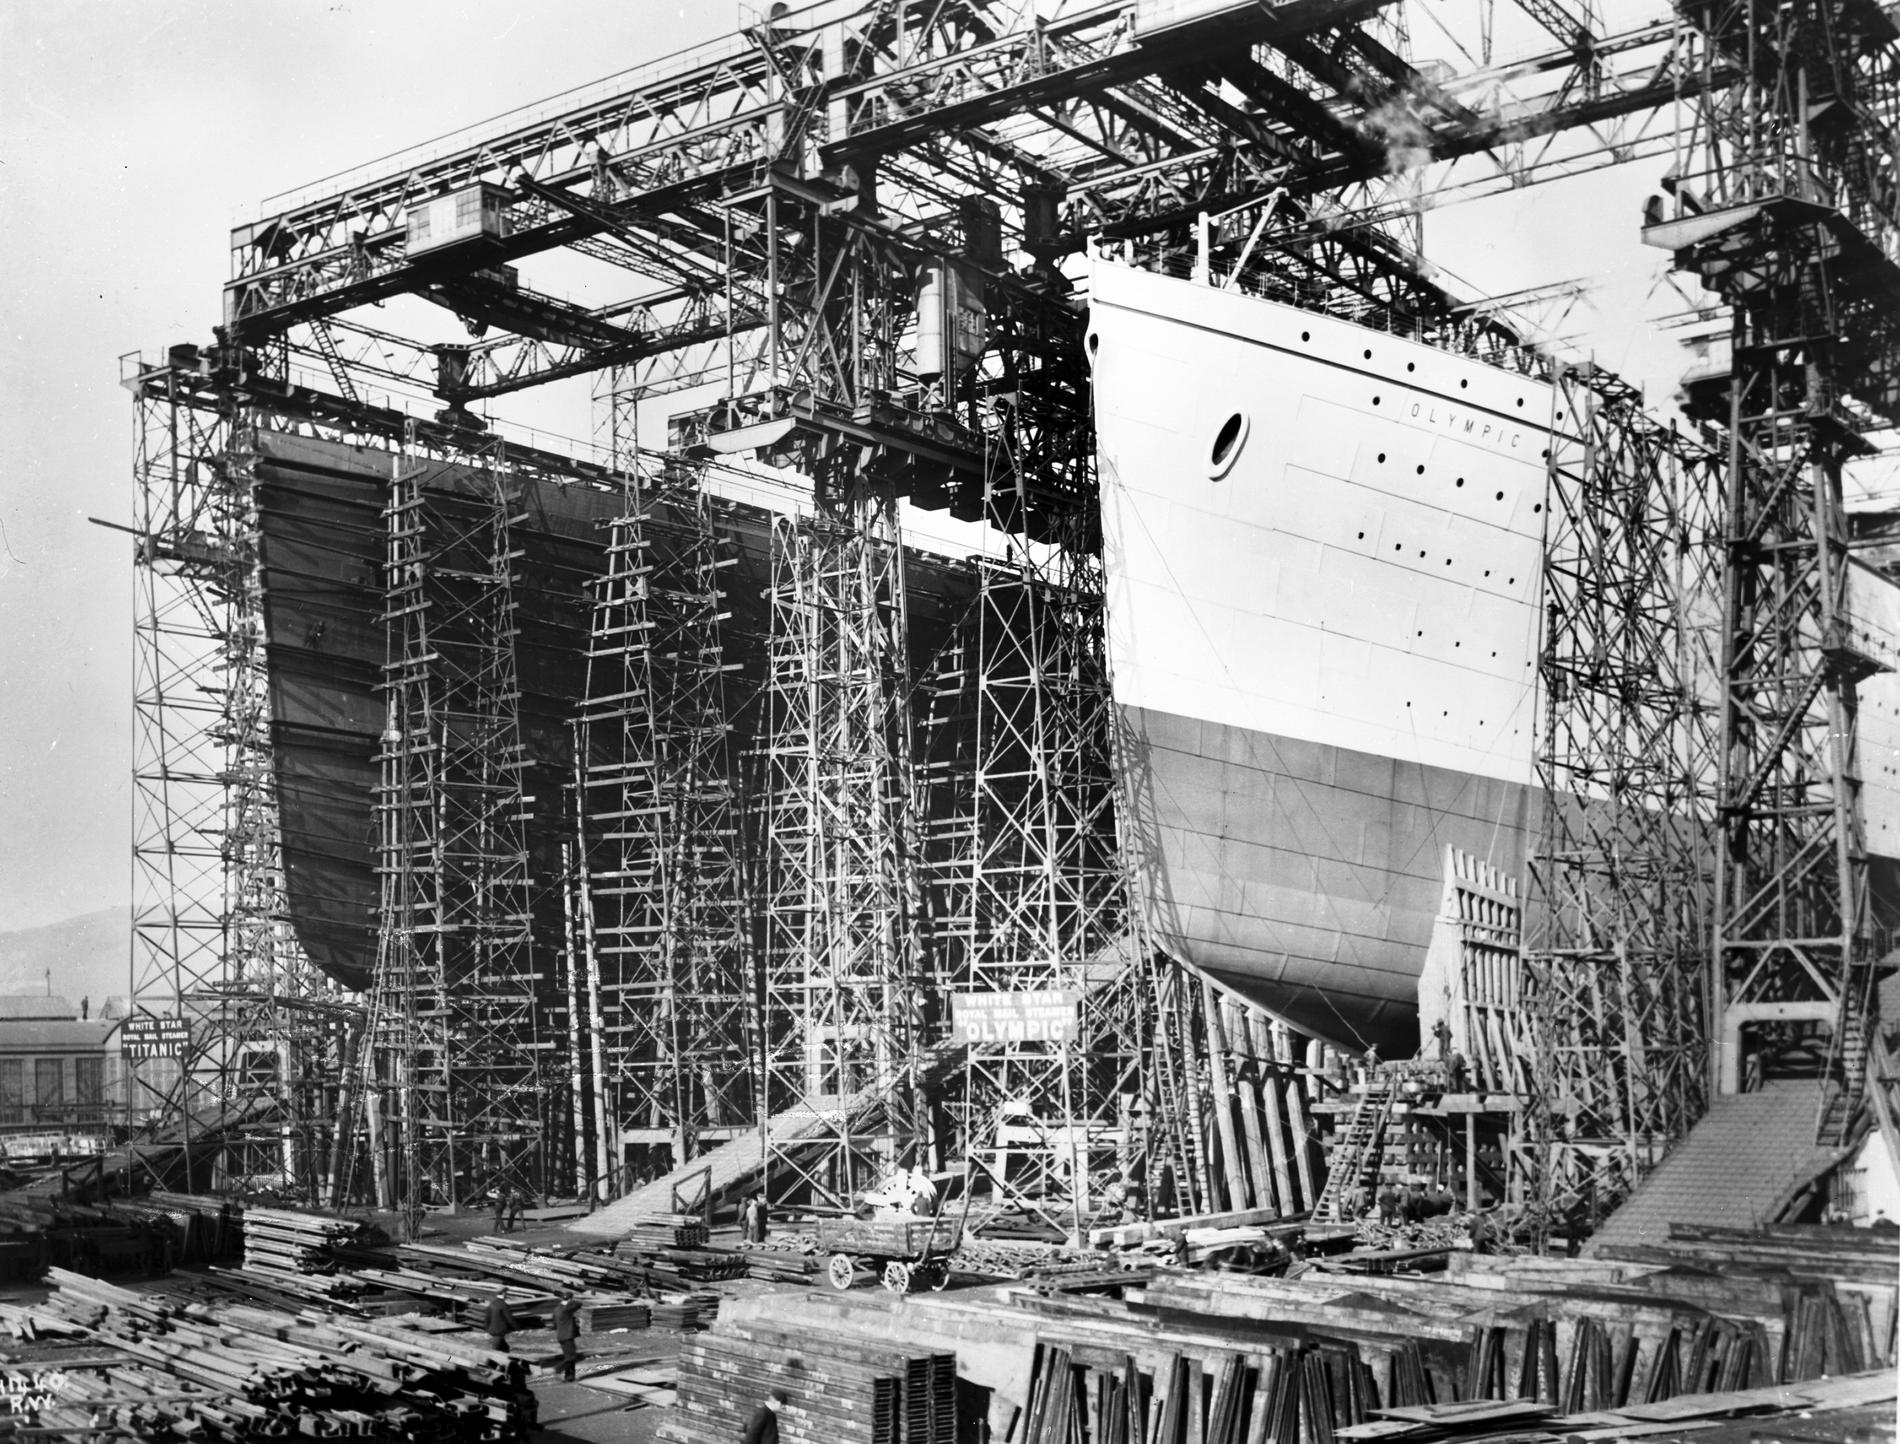
\includegraphics[height = 0.8\textheight]{olympic-titanic.jpg}
    \end{center}
    \note {
        What are we \emph{really} talking about here?
    }
\end{frame}

\section{Build everything}

\begin{frame}[fragile]
    \begin{description}
        \item [Building] \verb|python3 setup.py build|
        \item [Testing]  \verb|python3 setup.py test|
    \end{description}
\end{frame}

\begin{frame}[fragile]
    \verb|python3 setup.py test| is still too manual
\end{frame}

\begin{frame}
    \begin{block}{Lesson learned}
        Things not done automatically will not be done
    \end{block}

    \note {
        In order to do things automatically for many systems, we need some
        scaffolding
    }
\end{frame}

\begin{frame}[fragile]{travis.yml}
    \inputminted[lastline=12]{yaml}{travis.yml}
\end{frame}

\begin{frame}[fragile]{travis.yml}
    \inputminted[firstline=16,lastline=25]{yaml}{travis.yml}
\end{frame}

\begin{frame}[fragile]{travis.yml}
    \inputminted[firstline=27]{yaml}{travis.yml}
\end{frame}

\begin{frame}
    \begin{tabular}{l l}
        Machine definition  & Service default + config \\
        Scripts             & Config, setup.py, cmake \\
        Triggers            & New HEAD \\
    \end{tabular}

    \note{
        \begin{itemize}
            \item A machine definition would be perfect for obsolete systems
                  like RHEL5 and Windows
            \item Multiple machine definitions means we can test on multiple
                  systems
            \item With triggers, they can now run on every PR and every HEAD
                  pushed
            \item A new release can also be a trigger
            \item Makes it easier for contributers too, they don't have to set
                  up a complicated rig to run the new changes on multiple
                  systems
            \item So what does it look like?
        \end{itemize}
    }
\end{frame}

\begin{frame}
    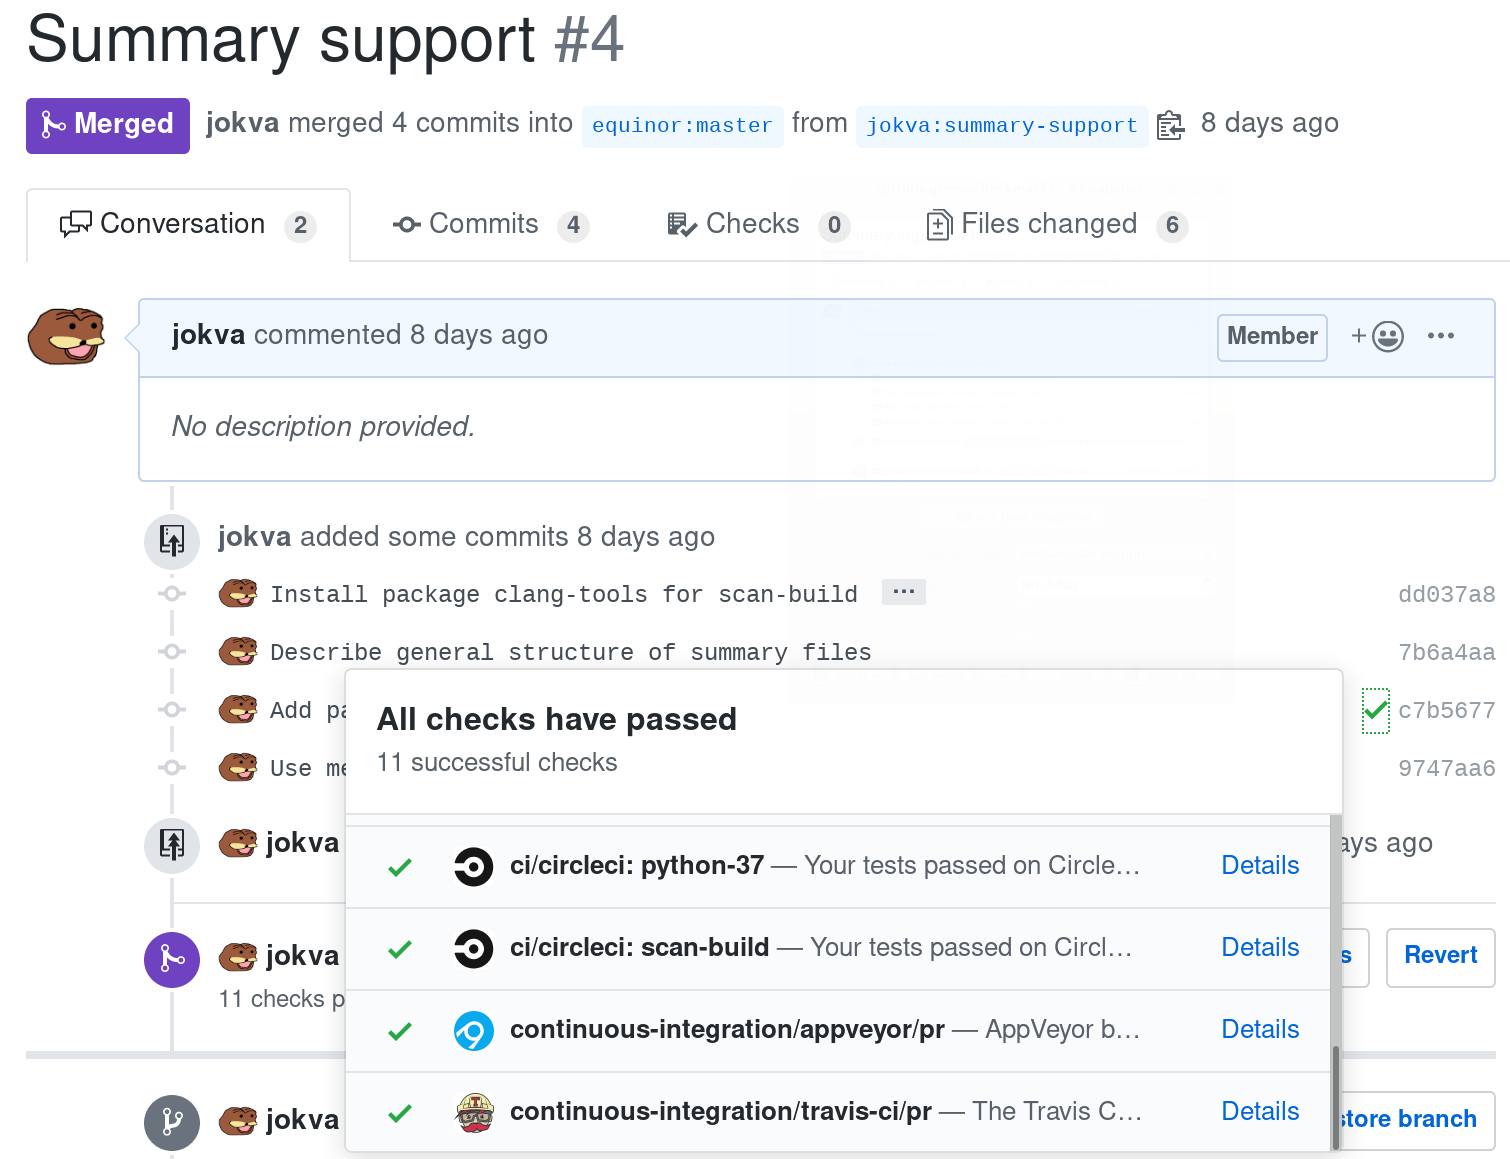
\includegraphics[width = \textwidth]{github-checks-passed.png}

    \note {
        \begin{itemize}
            \item We outsource this work to third-party services
            \item Travis, Circle, Appveyor, Gitlab, Pipelines
            \item Mostly configured in yaml with custom keys
            \item Fairly well documented
        \end{itemize}
    }
\end{frame}

\begin{frame}{}
    \begin{center}
        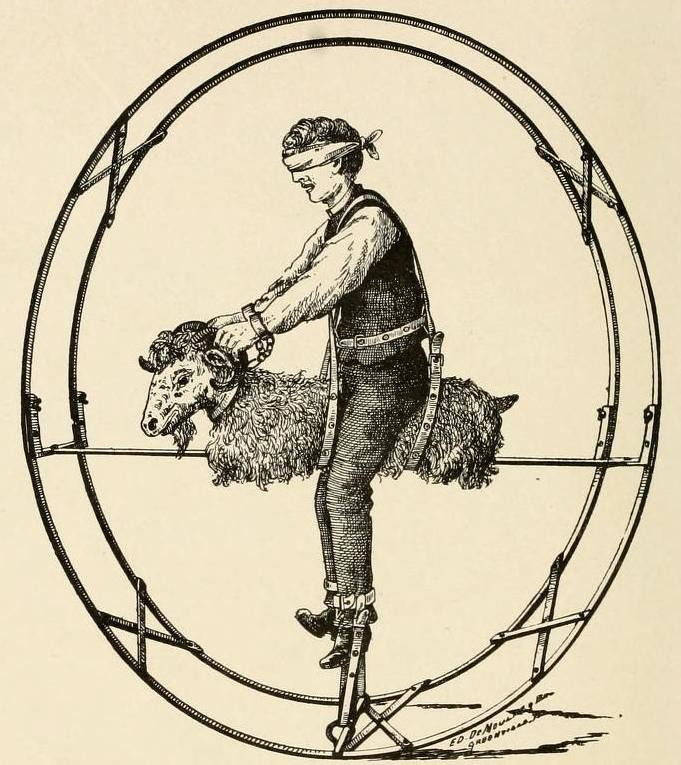
\includegraphics[height = 0.8\textheight]{reinvent-wheel.jpg}
    \end{center}
\end{frame}

\section{Reinventing the wheel}

\begin{frame}[fragile]
    \begin{block}{Wheel naming}
        \verb|{name}-{version}(-{build})?-{python}-{abi}-{plat}.whl|
    \end{block}

    \note{
        \begin{itemize}
            \item An ABI tag helps pip select the right package
            \item pip resolves these names from the host system
        \end{itemize}
    }
\end{frame}

\begin{frame}[fragile]
    \begin{block}{On Debian 10 (Buster)}
        \begin{minted}{bash}
$ python3 setup.py bdist_wheel
$ unzip -l dist/my_project-0.0.1-cp37-cp37m-linux_x86_64.whl
my_package/__init__.py
my_package/core.py
my_package/math.cpython-37m-x86_64-linux-gnu.so
my_project-0.0.1.dist-info/LICENSE
my_project-0.0.1.dist-info/METADATA
my_project-0.0.1.dist-info/WHEEL
my_project-0.0.1.dist-info/top_level.txt
my_project-0.0.1.dist-info/RECORD
        \end{minted}
    \end{block}

    \note{
        \begin{itemize}
            \item Notice the tag says linux. Not well suited for distribution
                  because users might have older libc
            \item For good binaries we need the manylinux tag
            \item OS X was omitted because it's quite long, but follows the
                  same pattern
            \item The manylinux image is specified by the PyPA, basically the
                  oldest libc + supporting libs they could use (RHEL5)
            \item Windows packages built on Windows, linux on RHEL5 etc
        \end{itemize}
    }
\end{frame}

\begin{frame}
    \begin{block}{Problem}
        No zlib on the user machine
    \end{block}

    \note {
        \begin{itemize}
            \item We'd still like the pip-package to \emph{just work}
            \item In particular an issue for fat wrappers around not-always
                  distributed libraries
        \end{itemize}
    }
\end{frame}

\begin{frame}
    \begin{block}{Solution}
        Distribute zlib with the wheel
    \end{block}
\end{frame}

\begin{frame}[fragile]
    \begin{minted}[highlightlines={7-11}]{bash}
$ auditwheel repair dist/my_project-0.0.1-cp37-cp37m-linux_x86_64.whl
Fixed-up wheel written to wheelhouse/
    \end{minted}
\end{frame}

\begin{frame}[fragile]
    \begin{minted}[highlightlines={5-9}]{bash}
$ unzip -l wheelhouse/my_project-0.0.1-cp37-cp37m-linux_x86_64.whl
my_package/__init__.py
my_package/core.py
my_package/math.cpython-35m-x86_64-linux-gnu.so
my_package/.libs/libstdc++-4376550d.so.6.0.22
my_package/.libs/libc-2-d37be6b0.24.so
my_package/.libs/libm-2-bfba5a97.24.so
my_package/.libs/libgcc_s-41124e5d.so.1
my_package/.libs/libz-7fd423a0.so.1.2.8
my_project-0.0.1.dist-info/RECORD
my_project-0.0.1.dist-info/top_level.txt
my_project-0.0.1.dist-info/METADATA
my_project-0.0.1.dist-info/WHEEL
    \end{minted}
\end{frame}

\section{It wasn't me}

\begin{frame}
    \begin{block}{Problem}
        Binary incompatibility - still not redistributable
    \end{block}
\end{frame}

\begin{frame}[fragile]
    \begin{block}{On Red Hat 5}
        \begin{minted}{bash}
$ python3 setup.py bdist_wheel
$ ls dist/
my_project-0.0.1-cp37-cp37m-manylinux1_x86_64.whl
        \end{minted}
    \end{block}
\end{frame}

\begin{frame}
    \begin{block}{Problem}
        No machine running Windows
    \end{block}
\end{frame}

\begin{frame}
    \begin{block}{Problem}
        No machine running Red Hat 5
    \end{block}
\end{frame}

\begin{frame}[fragile]
    \begin{minted}{yaml}
deploy:
    - provider: pypi
      skip_cleanup: true
      skip_upload_docs: true
      skip_existing: true
      user: statoil-travis
      distributions: --skip-cmake build sdist
      password:
        secure: encrypted-key
      on:
        tags: true
    \end{minted}
\end{frame}

\begin{frame}[fragile]
    \verb|python3 -m pip install my-project|
\end{frame}

\begin{frame}
    \begin{center}
        
\includegraphics[height = 0.8\textheight]{mechazawa-dist.png}
    \end{center}
\end{frame}

\section{Summary}

\begin{frame}
    \begin{itemize}
        \item Created a package
        \item Built extension on multiple platforms
        \item Assembled wheel with bundled dependencies
        \item Automatically tested and published package
    \end{itemize}
\end{frame}

\begin{frame}{Shoutout}
    \begin{description}
        \item [scikit-build] Setuptools-CMake glue
        \item [multibuild] Wheel automation
    \end{description}
\end{frame}

\begin{frame}
    Questions?
\end{frame}

\end{document}
